\documentclass[xcolor=dvipsnames,14pt,professionalfonts]{beamer}
\usepackage{minted}
\usepackage{etoolbox}
\usepackage[T1]{fontenc}
\usepackage{lmodern}
\usepackage[no-math]{fontspec} 
\usetheme{rsmarttraining}
\usefonttheme{professionalfonts}
\usecolortheme{dolphin}

%\definecolor{foreground}{gray}{0}
%\definecolor{background}{gray}{1}
%\definecolor{keyword}{rgb}{0.2,0.2,0.8}
%\definecolor{warning}{rgb}{0.8,0.2,0.2}
%\definecolor{shadow}{gray}{0.35}
%\definecolor{hide}{gray}{0.9}
%\definecolor{figure}{rgb}{1,0.7,0}
%\definecolor{title}{rgb}{25,240,250}
\definecolor{title}{rgb}{0.09,0.30,0.38}
\definecolor{frametitle}{rgb}{1,1,1}
\definecolor{normal}{rgb}{0,0,0}

%\usecolortheme[named=keyword]{structure}

\setbeamercolor{title}{fg=title}
\setbeamercolor{frametitle}{fg=frametitle}
\setbeamercolor{section in toc}{fg=foreground}
\setbeamercolor{normal text}{bg=brown!46,fg=normal}

\setbeamerfont{structure}{family=\fontspec{Georgia},series=\bfseries} 
\setbeamerfont{subtitle}{family=\fontspec{Helvetica},series=\bfseries} 
\begin{document}

\title{KRAD Training}
\subtitle{Exercise: Javascript and AJAX}
\author[Leo]{Leo Przybylski}

\usebackgroundtemplate%
{%
    
\includegraphics[width=\paperwidth,height=\paperheight]{../img/header.png}%
}

{
\usebackgroundtemplate{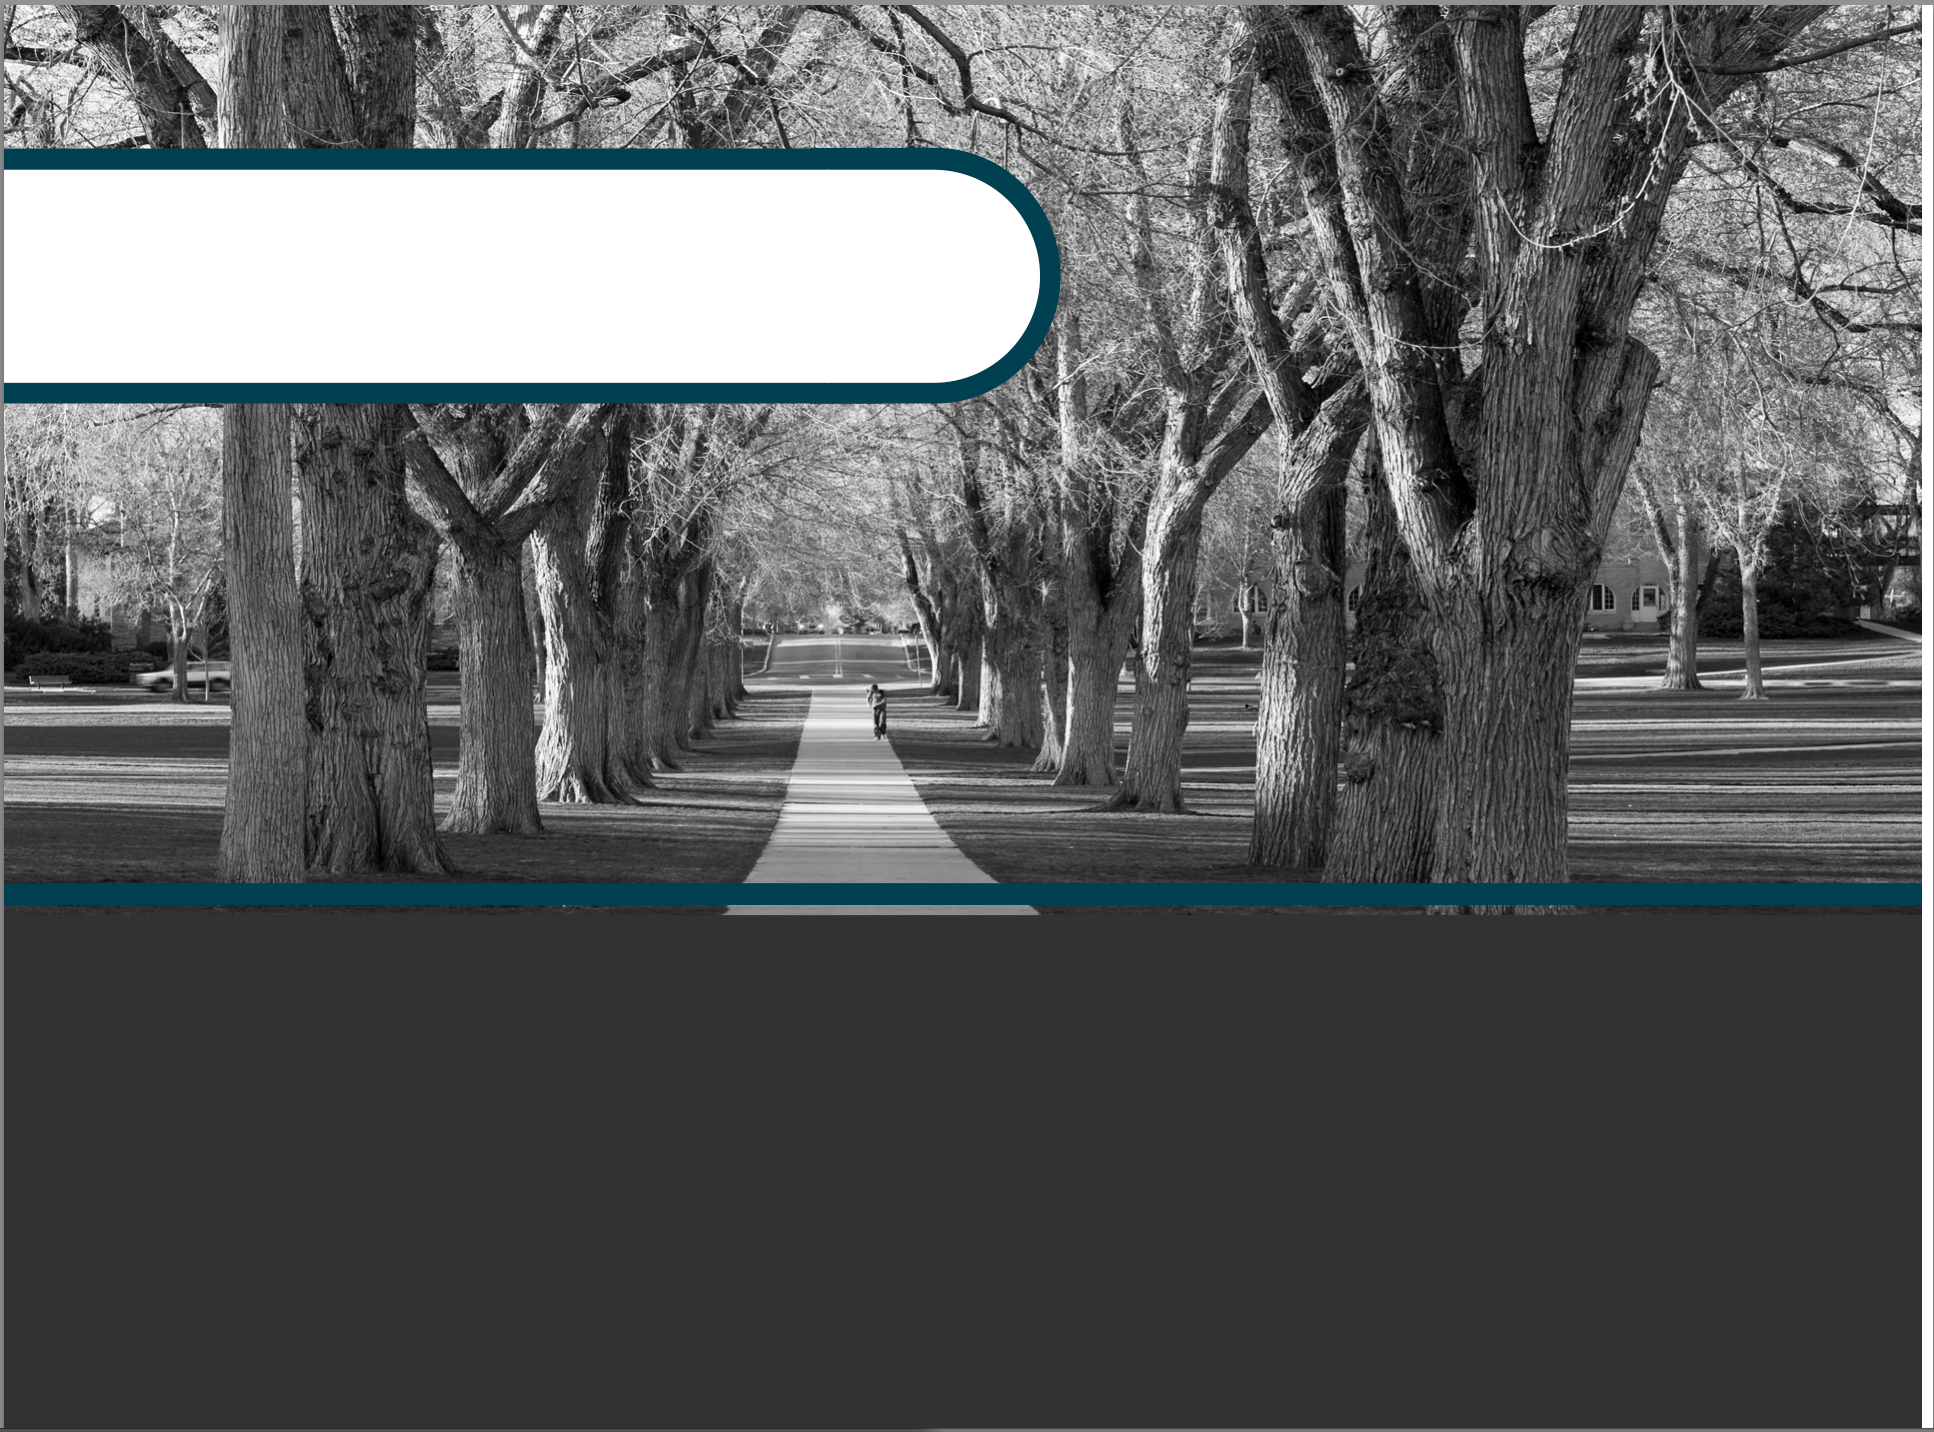
\includegraphics[width=\paperwidth]{../img/title.png}}%
\begin{frame}[plain]
  \titlepage
\end{frame}
}

\begin{frame}{Goals}
  \begin{itemize}
    \item Learn about creating ReST services.
    \item Exposing rest services on the service bus.
    \item Access the service via javascript.   
  \end{itemize}
\end{frame}

\begin{frame}{Instructions}
  \begin{enumerate}
  \item Create a service that returns a list of covers.
  \item Export the service to the service bus.
  \item Verify that the service is exported to the service bus.
  \item Create a javascript function to retrieve the covers.
  \end{enumerate}
  \end{frame}

\begin{frame}[fragile]{CoverServiceImpl}
  \begin{enumerate}
    \item Create a new class in the \textbf{trnapp.bookstore} package
    \begin{minted}[fontsize=\scriptsize]{java}
@Path("/")
@Produces(MediaType.APPLICATION_JSON)
public class CoverServiceImpl {

}
\end{minted}
\end{enumerate}
\end{frame}

\begin{frame}{CoverServiceImpl}
  \begin{itemize}
    \item The \textbf{Path} annotation maps the service to
      \texttt{remoting/coverService}
    \item Another \textbf{Produces} annotation is added so the service
      bus will invoke the JSON provider because the content type is JSON.
  \end{itemize}
\end{frame}

\begin{frame}[fragile]{CoverServiceIMpl}
  \begin{enumerate}
    \item Add a method to retrieve cover data
    \begin{minted}[fontsize=\scriptsize]{java}
    @GET
    @Path("/Covers")
    @Produces(MediaType.APPLICATION_JSON)
    public Response getCovers() {    	    	
    	return Response.ok(new Results()).build();
    }
\end{minted}
\end{enumerate}
\end{frame}

\begin{frame}[fragile]{CoverServiceIMpl}
  \begin{enumerate}
  \item Our method to retrieve covers uses a \textbf{Results} class. 
  \item Create it.
    \begin{minted}[fontsize=\scriptsize]{java}
@XmlRootElement
@XmlAccessorType(XmlAccessType.FIELD)
@XmlType(name = "", propOrder = {"covers"})
static final class Results {
}
\end{minted}
\item XmlRootElement, XmlAccessorType, and XmlType annotations are
  used so this class can be converted to JSON by a JAXB provider like
  Jettison which comes with CXF.
\end{enumerate}
\end{frame}

\begin{frame}[fragile]{CoverServiceIMpl}
  \begin{enumerate}
    \item Next we add properties like a list over covers to our
      results. For now, we are hard-coding covers until we can inject
      a service later that will retrieve them.
    \begin{minted}[fontsize=\scriptsize]{java}
@XmlElement
protected List<Cover> covers;
	
public Results() {
	covers = new ArrayList<Cover>();
	covers.add(new Cover(1L, "/trnapp/images/cover1.png"));
	covers.add(new Cover(2L, "/trnapp/images/cover2.png"));
	covers.add(new Cover(3L, "/trnapp/images/cover3.png"));
	covers.add(new Cover(4L, "/trnapp/images/cover4.png"));
	covers.add(new Cover(5L, "/trnapp/images/cover5.png"));
	covers.add(new Cover(6L, "/trnapp/images/cover6.png"));
}
\end{minted}
\end{enumerate}
\end{frame}

\begin{frame}[fragile]{Covers}
  \begin{enumerate}
    \item Since we're using JAXB to convert java objects to JSON, we
      need a Cover class for all cover instances.
    \begin{minted}[fontsize=\scriptsize]{java}
@XmlRootElement
@XmlAccessorType(XmlAccessType.FIELD)
@XmlType(name = "", propOrder = {
        "bookId", "imageUrl" })
public class Cover {
	@XmlElement
	private Long bookId;
	@XmlElement
	private String imageUrl;

}
\end{minted} 
\end{enumerate}
\end{frame}

\begin{frame}[fragile]{Covers}
  \begin{enumerate}
    \item The \textbf{Cover} class has two properties
      \begin{itemize}
        \item bookId
          \item imageUrl
        \end{itemize}
      \item these properties will be used to map books to a URL for
        the cover image
\end{enumerate}
\end{frame}


\begin{frame}[fragile]{Register the with Spring}
  \begin{enumerate}
    \item Now we need to tell Spring about the service
    \begin{minted}[fontsize=\scriptsize]{xml}
<bean id="coverService" class="trnapp.bookstore.CoverServiceImpl" />
\end{minted} 
\end{enumerate}
\end{frame}
    
\begin{frame}[fragile]{Create a RestDefinition for the Service}
  \begin{enumerate}
    \item This may seem redundant with the JAX-RS annotations, but we
      still need to define the service as a ReST service with Rice.
    \begin{minted}[fontsize=\scriptsize]{xml}
    <bean id="CoverService" class="org.kuali.rice.ksb.api.bus.support.RestServiceDefinition">
      <property name="serviceNameSpaceURI" value="http://rice.kuali.org/krad/v2_0"/>
      <property name="service" ref="coverService"/>
      <property name="resourceClass"
                value="trnapp.bookstore.CoverServiceImpl"/>
      <property name="localServiceName" value="coverService"/>
      <property name="providers">
        <list>
          <bean class="org.apache.cxf.jaxrs.provider.json.JSONProvider" /> 
        </list>
      </property>
      <property name="extensionMappings">
        <map>
          <entry key="xml" value="application/xml"/>
          <entry key="json" value="application/json"/>
          <entry key="html" value="text/html"/>
          <entry key="xhtml" value="application/xhtml+xml"/>
        </map>
      </property>
    </bean>
\end{minted} 
\end{enumerate}
\end{frame}
    
 \begin{frame}[fragile]{Export the Service to the Service Bus}
  \begin{enumerate}
    \item The service still isn't available on the service bus. To do
      this, we use the \textbf{ServiceBusExporter} with our newly
      created \textbf{RestServiceDefinition} bean
    \begin{minted}[fontsize=\scriptsize]{xml}
   <bean class="org.kuali.rice.ksb.api.bus.support.ServiceBusExporter">
      <property name="serviceBus" ref="rice.ksb.serviceBus"/>
      <property name="serviceDefinition" ref="CoverService"/>
    </bean>
    \end{minted}
    \end{enumerate}
\end{frame}

 \begin{frame}[fragile]{Verify the Service is Exported}
  \begin{enumerate}
    \item Start Jetty
    \item Go to the \textbf{Administration} Page
    \item Click on the \textbf{Service Registry} link
    \item Locate the \textbf{coverService}
      \item If you find it, it exported correctly; otherwise,
        something has gone wrong and you should review the steps once more.
    \end{enumerate}
\end{frame}

 \begin{frame}[fragile]{Verify the Service is Exported}
  \begin{enumerate}
  \item The service should have a URL that looks something like
    \textbf{http://localhost:8080/trnapp/remoting/coverService/Covers}
  \item If you access the URL directly, you should see the following
    results:
        \begin{minted}[fontsize=\scriptsize]{xml}
{"results":{"covers":[{"bookId":1,"imageUrl":"\/trnapp\/images\/cover1.png"},{"bookId":2,"imageUrl":"\/trnapp\/images\/cover2.png"},{"bookId":3,"imageUrl":"\/trnapp\/images\/cover3.png"},{"bookId":4,"imageUrl":"\/trnapp\/images\/cover4.png"},{"bookId":5,"imageUrl":"\/trnapp\/images\/cover5.png"},{"bookId":6,"imageUrl":"\/trnapp\/images\/cover6.png"}]}}
          \end{minted}
    \end{enumerate}
\end{frame}

 \begin{frame}[fragile]{custom.js}
  \begin{enumerate}
    \item In \textbf{src/main/webapp/scripts}, there is a
      \textbf{custom.js} file that includes a sample JQuery function
      for retrieving data from the ReST service and populating a
      Bootstrap carousel with it.
    \begin{minted}[fontsize=\scriptsize]{xml}
 jQuery(document).ready(function() {
    var covers = []
    jQuery.ajax({
        url : '/trnapp/remoting/coverService/Covers
        }).done(function(data) {
            covers = JSON.parse(data).results

            console.log("Covers are " + covers)
            console.log(jQuery('.carousel-inner > div.item > img'))
            jQuery('.carousel-inner > div.item > img').each(function(index, item) {
                console.log('setting cover to ' + covers[index])
                jQuery(item).attr('src', covers[index].imageUrl)
            });    

        });        
})
          \end{minted}
    \end{enumerate}
\end{frame}
\end{document}
